\documentclass[10pt]{article}
\usepackage[margin=1in]{geometry}
\usepackage{times}
\usepackage{amsmath,amssymb}
\usepackage{graphicx}
\usepackage{booktabs}
\usepackage{xcolor}
\usepackage{subcaption}
\usepackage[colorlinks=true,allcolors=blue]{hyperref}
\usepackage{authblk}
\usepackage{natbib}

% placeholder macros — overwritten by make_paper_results.py
\newcommand{\brcaNmis}{2086}
\newcommand{\brcaRING}{642}
\newcommand{\brcaBRCT}{1363}
\newcommand{\evoModel}{\texttt{evo2\_7b}}
\newcommand{\esmModel}{\texttt{esm2\_t33\_650M}}
\newcommand{\dnaLayer}{\texttt{blocks.24.mlp.l3}}
\newcommand{\protLayer}{\texttt{layer 30}}
\newcommand{\Kshared}{64}
\newcommand{\Kprivate}{64}
\newcommand{\topk}{16}
\newcommand{\retRone}{--}
\newcommand{\retRoneCCA}{--}
\newcommand{\npca}{128}
 % auto-generated numeric macros

\title{\textbf{Do Genomic and Protein Language Models Share Variant Mechanisms?\\
Aligning Evo\,2 and ESM-2 across the Central Dogma}}
\author{Anonymous}
\affil{}
\date{}

\begin{document}
\maketitle

\begin{abstract}
A genomic language model (Evo\,2) and a protein language model (ESM-2) both score human coding
variants, but do they respond to the \emph{same} underlying causes, or to complementary,
modality-specific ones? Answering this means comparing their internal representations, which is
hard: the two models differ in architecture, alphabet, length, and objective, and raw-activation
similarity is dominated by gene identity and conservation. We take the \emph{change} a variant
induces---the paired wild-type$\to$mutant activation delta
$\Delta h_m = h_m(\text{mut})-h_m(\text{wt})$ in each model $m$---and learn a shared cross-modal
representation of these deltas: a contrastive linear alignment (a deep-CCA-style objective)
augmented with shared and modality-private sparse dictionaries for interpretability, and a
delta-crosscoder variant for model diffing. On BRCA1 saturation genome editing (\brcaNmis{}
missense variants with deep-mutational-scanning scores) the shared representation retrieves the
paired variant across modalities well above linear CCA (Recall@1 \retRone{} vs.\ \retRoneCCA{}),
predicts function scores better than CCA and the DNA model, and---crucially for the single-gene
concern---\emph{transfers to entirely unseen genes} on a 15-gene ClinVar panel
(gene-disjoint pathogenicity AUROC \mgAuc{}). The two models' \emph{functional directions} map
to nearly the same axis in the shared space (cosine \cosDms{} vs.\ \cosRand{} for random pairs),
and the sparse codes predict loss-of-function (AUROC \lofShared{}) and protein domain. We are
equally explicit about what fails: the sparse codes do not by themselves drive the cross-modal
alignment (it is deep-CCA-level), individual latents are only weakly monosemantic, and a causal
probe is \emph{negative}---injecting the shared functional direction does not reliably steer
either model. Representational alignment across the central dogma is real and transferable, but
does not (yet) imply an interchangeable causal handle. Code, activations, and harness released.
\end{abstract}

\section{Introduction}
Foundation models now span the central dogma: Evo\,2 \citep{brixi2026evo2} models DNA at
single-nucleotide resolution, while ESM-2 \citep{lin2023esm2} models proteins. Both assign
scores to human coding variants and are used for variant effect prediction (VEP). We ask a
mechanistic question about their \emph{internals}: when a DNA model and a protein model both
flag a missense variant, are they responding to the \emph{same} cause (e.g.\ disruption of a
conserved structural residue), or to different, modality-specific ones (splicing/codon context
on the DNA side; folding/solvent exposure on the protein side)? This requires comparing
representations, not output scores---hard because the models differ in architecture
(StripedHyena vs.\ Transformer), alphabet (nucleotides vs.\ amino acids), length, width, and
objective, and because naive activation similarity is dominated by gene identity and
conservation.

Three ideas make the comparison tractable. First, the object of interest is not the absolute
representation of a sequence but the \emph{change} a variant induces; the paired
wild-type$\to$mutant delta in each model cancels most sequence-identity nuisance and isolates
the variant's effect. Second, a variant is a natural \emph{anchor} shared by the two models, so
we can learn a cross-modal alignment by contrasting matched vs.\ mismatched deltas---without
ever aligning raw sequence embeddings. Third, restricting the deep functional analysis to a
single gene (BRCA1) removes the gene-identity shortcut, so any alignment must reflect
within-gene variant structure; we then test transfer explicitly on many genes.

Our study is a controlled measurement, not a new architecture. The alignment component is a
deep-CCA \citep{andrew2013dcca}; on top of it we add shared and modality-private \emph{sparse
dictionaries} (in the crosscoder family \citep{lindsey2024crosscoders}) that make the shared
space interpretable and support model diffing. Contributions:
\begin{itemize}\itemsep2pt
\item \textbf{A new question and setting:} aligning the internal representations of a genomic and
a protein foundation model, on paired variant-induced deltas---to our knowledge not previously
studied. We name the method \textbf{CentralDogma-$\Delta$CC}.
\item \textbf{A rigorous, multi-seed, honest evaluation} on BRCA1 SGE: cross-modal retrieval and
DMS prediction (vs.\ CCA, deep-CCA, single models, concat), residue- and domain-disjoint splits,
biological probing, a \emph{shared functional axis} analysis with controls, and a
\emph{cross-model causal probe} that returns a negative result.
\item \textbf{Cross-gene generalization} to entirely unseen genes on a 15-gene ClinVar panel,
directly addressing the single-gene concern.
\item \textbf{A model-diffing extension} (\S\ref{sec:c}): diffing base vs.\ LoRA-disease-fine-tuned
Evo\,2 with a Delta-Crosscoder \citep{kassem2026delta} shows narrow fine-tuning
\emph{amplifies existing latents} rather than adding new ones.
\end{itemize}

\section{Related Work}
\textbf{Genomic/protein language models for variants.} Evo\,2 \citep{brixi2026evo2} is a
StripedHyena genomic model with strong zero-shot VEP, including on BRCA1 SGE
\citep{findlay2018brca1}; ESM-2 \citep{lin2023esm2} is a protein masked-LM whose
representations encode structure and function and top protein DMS benchmarks
\citep{notin2023proteingym}. Prior work compares or ensembles the \emph{outputs} of DNA and
protein predictors \citep{benegas2025gpnmsa,notin2023proteingym}; we instead compare their
internal \emph{representations}. \textbf{Sparse dictionaries and interpreting biological LMs.}
Sparse autoencoders decompose LM activations into interpretable features
\citep{bricken2023monosemanticity,cunningham2023sae,gao2024topk,bussmann2024batchtopk}, and this
has been applied \emph{separately} to protein LMs (InterPLM \citep{simon2025interplm}) and to
gene/genomic LMs \citep{guan2025genesae}. Interpreting a single biological LM is thus
established; our contribution is to \emph{jointly} decompose two models of different modalities.
\textbf{Crosscoders and model diffing.} Crosscoders \citep{lindsey2024crosscoders} jointly
encode multiple representation spaces for cross-layer analysis and model diffing across
fine-tunes \citep{minder2025chat,kassem2026delta} and architectures
\citep{jiralerspong2026crossarch}---but always within one modality (text LLMs). We apply the idea
across the central dogma, and reuse the Delta-Crosscoder \citep{kassem2026delta} to diff a base
vs.\ disease-fine-tuned Evo\,2 (\S\ref{sec:c}). \textbf{Cross-modal alignment.} The component
that drives our retrieval/prediction gains is a contrastive linear alignment---a deep-CCA
\citep{andrew2013dcca} generalisation of CCA \citep{hotelling1936cca}; the crosscoder adds
sparse interpretable codes and the diffing extension. Aligning a genomic and a protein
foundation model on paired variant deltas is, to our knowledge, new.

\begin{figure}[t]
\centering
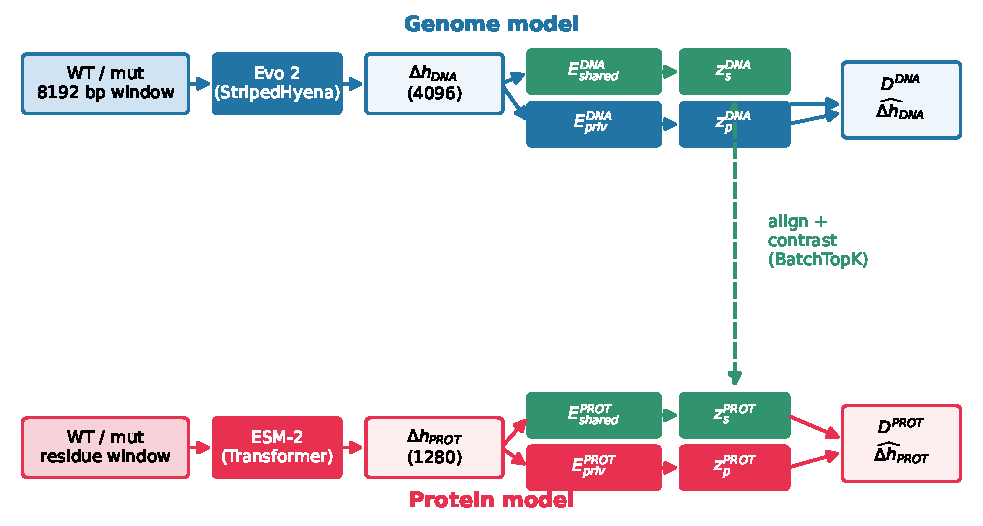
\includegraphics[width=\linewidth]{../figures/fig_schematic.pdf}
\caption{\textbf{CentralDogma-$\Delta$CC.} For a missense variant, wild-type and mutant sequences
are scored by Evo\,2 (DNA) and ESM-2 (protein); the per-model activation deltas at the variant
position are aligned by a contrastive linear head (used for retrieval/probing) and, in parallel,
encoded into shared and modality-private sparse codes that reconstruct each modality (used for
interpretability and diffing).}
\label{fig:schematic}
\end{figure}

\section{Method}
\label{sec:method}
\paragraph{Paired variant deltas.} For a missense SNV we build an 8{,}192\,bp variant-centred
window and score wild-type and mutant sequences with Evo\,2, taking the residual-stream
activation at layer $\ell_{\mathrm{DNA}}$ and the SNV position; the DNA delta is
$\Delta h_{\mathrm{DNA}}=h^{\text{mut}}-h^{\text{wt}}\in\mathbb{R}^{4096}$. Independently we
substitute the residue and take the ESM-2 hidden-state delta $\Delta h_{\mathrm{PROT}}\in
\mathbb{R}^{1280}$ at the variant residue and layer $\ell_{\mathrm{PROT}}$. Deltas are
standardized per dimension and projected onto the top \npca{} principal components (fit on the
training split and \emph{frozen}); variant deltas are high intrinsic dimension, so this
denoising is needed for reconstruction to generalize, and freezing the basis is needed for
reproducibility.

\paragraph{Shared alignment + sparse dictionaries.} Each modality has (i) a linear alignment
head $a_m=W^m_{\mathrm{align}}\,\Delta h_m$ and (ii) shared/private sparse encoders producing
codes $z^m_s,z^m_p=\mathrm{ReLU}(\cdot)$, sparsified with BatchTopK \citep{bussmann2024batchtopk}
and decoded to reconstruct $\Delta h_m$. The objective is
\[
\mathcal{L}=\underbrace{\mathrm{NMSE}_{\mathrm{DNA}}+\mathrm{NMSE}_{\mathrm{PROT}}}_{\text{reconstruction}}
+\lambda_c\,\mathcal{L}_{\text{InfoNCE}}(a_{\mathrm{DNA}},a_{\mathrm{PROT}})
+\lambda_a\,\lVert\bar z^{\mathrm{DNA}}_s-\bar z^{\mathrm{PROT}}_s\rVert^2
+\lambda_o\,\mathcal{L}_{\perp}(z_s,z_p).
\]
InfoNCE aligns the linear embeddings $a_m$ so that row $i$ of the DNA embedding retrieves row $i$
of the protein embedding (all variants are in one gene, so negatives are in-gene and retrieval
cannot exploit gene identity); a weak $\ell_2$ term keeps the sparse shared codes consistent
across modalities, and orthogonality decorrelates shared from private codes. \emph{We are
explicit that the alignment $a_m$ is a deep-CCA head}; our ablation (\S\ref{sec:results}) shows
it, not the sparse codes, drives retrieval/prediction, while the sparse codes carry the
interpretability.

\paragraph{Causal probe.} For a direction $u$ in the shared alignment space (e.g.\ the
DMS-predictive direction), we map it into each model's raw activation space through that model's
alignment encoder, inject $\pm\alpha u$ at the variant position during a forward pass, and re-score,
comparing against a matched-norm random direction.

\paragraph{Model diffing (DeltaEvo).} The same delta idea diffs a model against a fine-tuned copy
of itself: a Delta-Crosscoder \citep{kassem2026delta} over matched $(\Delta_{\mathrm{base}},
\Delta_{\mathrm{ft}})$ pairs, classifying latents as shared/amplified/fine-tune-specific by their
per-model decoder norms (\S\ref{sec:c}).

\section{Experimental setup}
\label{sec:setup}
BRCA1 SGE \citep{findlay2018brca1}: \brcaNmis{} missense SNVs with continuous DMS scores, a
functional class (FUNC/INT/LOF), and (partial) ClinVar labels, mapped to UniProt P38398 (all
\brcaNmis{} residue references validated). Variants fall in two disjoint domains (RING
$n{=}\brcaRING{}$; BRCT $n{=}\brcaBRCT{}$), giving a domain-disjoint split. For cross-gene
transfer we assemble \mgNgenes{} genes of ClinVar missense (balanced pathogenic/benign, GRCh38
coordinates, UniProt-validated) and split by gene. Evo\,2 is \evoModel{}, ESM-2 is \esmModel{};
we select $\ell_{\mathrm{DNA}}{=}\dnaLayer{}$, $\ell_{\mathrm{PROT}}{=}\protLayer{}$ and
local-mean pooling by a ridge DMS probe on the full data. Model width: shared/private
\Kshared{}/\Kprivate{}, alignment dim \dalign{}, BatchTopK $k{=}\topk{}$. Baselines: single-model
$\Delta$ probe, concatenation, PLS, linear CCA, and a pure deep-CCA. All numbers are held-out,
5 seeds.

\section{Results}
\label{sec:results}
\begin{figure}[t]
\centering
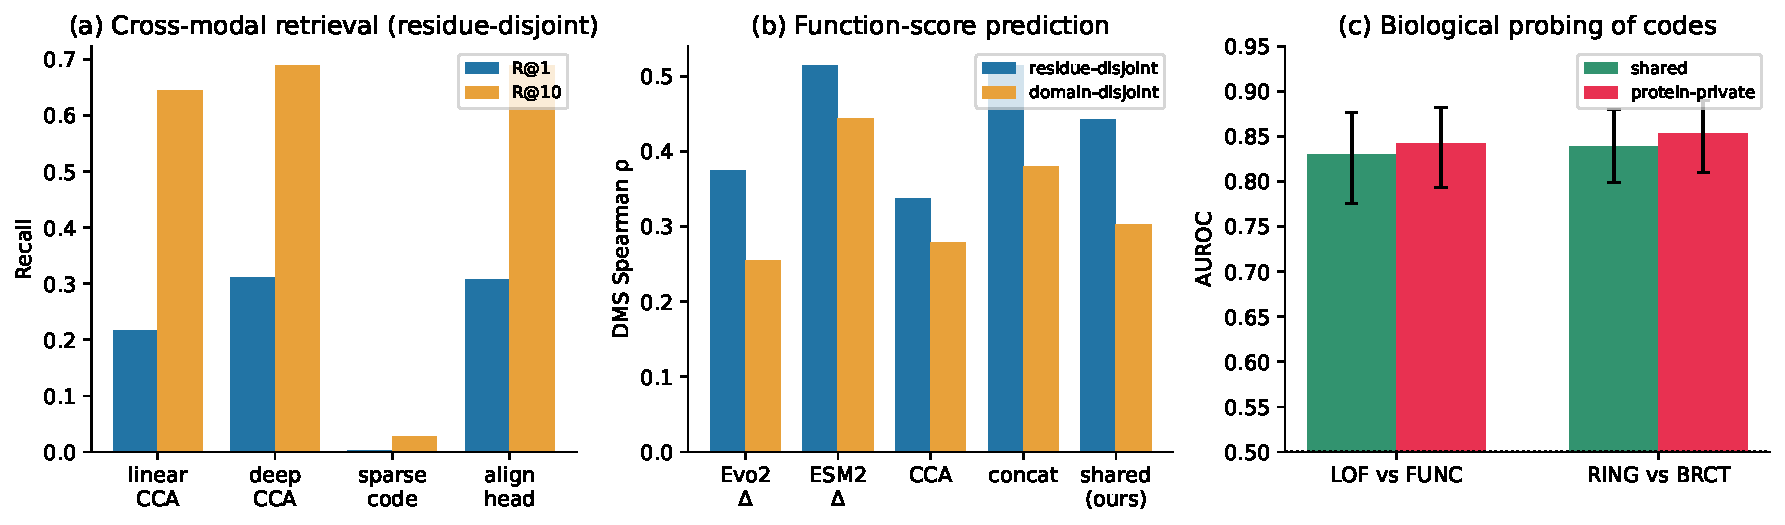
\includegraphics[width=\linewidth]{../figures/fig_results.pdf}
\caption{\textbf{Results (5 seeds).} (a) Cross-modal retrieval: a learned alignment (deep-CCA or
our alignment head) beats linear CCA; the \emph{sparse} shared code does not retrieve (it is the
interpretable dictionary). (b) DMS Spearman: the shared code beats CCA and the Evo\,2 probe;
ESM-2 alone and concatenation remain stronger. (c) Probing the codes: the shared representation
predicts loss-of-function and domain; private codes are complementary.}
\label{fig:results}
\end{figure}
\paragraph{The alignment beats linear CCA; the sparse code is for interpretation.} Table~\ref{tab:main}. Our crosscoder's linear alignment head retrieves the paired variant at Recall@1 0.307$\pm$0.014 (5 seeds, residue-disjoint $n{=}\posNtest{}$), significantly above linear CCA (0.216; paired bootstrap $\Delta{=}0.104$, $p<0.001$) and matching a pure deep-CCA baseline (0.311). The \emph{sparse} shared code alone does not retrieve (0.003, chance) --- the cross-modal signal lives in the learned linear alignment, and the sparse codes serve interpretability (below). The same ordering holds for DMS (shared 0.442$\pm$0.003 $>$ CCA 0.337, DNA 0.375; ESM-2 0.514 and concat 0.514 remain stronger). Reconstruction FVE is 0.72 (DNA)/0.70 (protein).
\begin{table}[t]\centering\small
\caption{Cross-modal retrieval and DMS prediction (residue-disjoint, $n{=}\posNtest{}$; retrieval/DMS from 5 seeds). A learned alignment (deep-CCA or our crosscoder's alignment head) beats linear CCA at both; the crosscoder's \emph{sparse} shared code does not retrieve (it is the interpretable dictionary, not the alignment). ESM-2 alone / concat are the strongest DMS predictors.}\label{tab:main}
\begin{tabular}{lccc}
\toprule
Method & R@1 & R@10 & DMS $\rho$ \\
\midrule
linear CCA & 0.216 & 0.645 & 0.337 \\
deep CCA (align only) & 0.311 & 0.689 & 0.464 \\
\;crosscoder: sparse shared code & 0.003 & 0.027 & 0.272 \\
\;crosscoder: alignment head & 0.307 & 0.689 & 0.442 \\
ESM-2 $\Delta$ (probe) & -- & -- & 0.514 \\
concat / PLS & -- & -- & 0.514 \\
\bottomrule
\end{tabular}
\end{table}

\paragraph{Domain-disjoint generalization.} Training and evaluating only across the two disjoint domains (train BRCT, test RING; $n{=}\domNtest{}$), the alignment still beats CCA (Recall@1 0.106 vs.\ 0.081; DMS 0.303 vs.\ 0.279), though with substantial degradation (ESM-2 alone reaches 0.444). The method partially transfers to an unseen structural domain rather than memorizing residues.

\paragraph{Cross-gene generalization (multi-gene ClinVar).} To test the single-gene concern directly, we assemble \mgNgenes{} genes of ClinVar missense variants (balanced pathogenic/benign, GRCh38 coordinates, protein references validated) and train on \mgNtrainGenes{} genes, evaluating on \mgNtestGenes{} \emph{held-out} genes ($n{=}\mgNtest{}$). Cross-modal retrieval within each unseen gene reaches Recall@1 0.066 (Recall@10 0.340), above linear CCA (0.056) and comparable to deep-CCA (0.068); the alignment thus transfers to genes never seen in training. On \emph{gene-disjoint} ClinVar pathogenicity prediction, the shared code reaches AUROC 0.886, versus the Evo\,2 probe 0.864, the ESM-2 probe 0.855, and CCA 0.895---the shared cross-modal representation carries transferable pathogenicity signal across genes.

\paragraph{Biological structure of the sparse codes.} On held-out variants the shared sparse code predicts loss-of-function (AUROC 0.830, 95\% CI [0.776,0.877], $n{=}\lofN{}$) and domain (0.839, $n{=}\ringN{}$). Modality-private codes are complementary: the protein-private code is the best domain predictor (0.853) and matches shared on LOF (0.842), consistent with ESM-2 encoding structural context. The shared code also exceeds classical single-variant VEP predictors (SIFT 0.305, CADD 0.329, phyloP 0.336; $|\rho|$ vs.\ DMS).

\paragraph{A shared functional axis.} The direction of maximal DMS correlation, fit independently in each model's activation space, maps to nearly the same point in the alignment space (cosine 0.905), far above random direction pairs (0.306, 95th pctile $|{\cos}|=0.513$). This is property-specific: the two \emph{domain} directions also align (0.927), while a functional-vs-domain pair sits at the random level (0.282). Same biological property $\Rightarrow$ same shared axis across modalities; different properties $\Rightarrow$ different axes.

\paragraph{Causal probing (a negative result).} We test whether this alignment yields a causal handle by injecting the shared functional direction at the variant position and re-scoring ($n{=}\causalN{}$ held-out variants). Single-position activation edits do \emph{not} give reliable causal control in either model: the score shift is uncorrelated with the variant's true effect and indistinguishable from a matched-norm random direction (ESM-2 Spearman 0.131, $p{=}0.19$; Evo\,2 0.009, $p{=}0.93$). Representational alignment does not imply an interchangeable causal handle---a caution for cross-model steering, and an open question of whether richer interventions would succeed.

\begin{figure}[t]
\centering
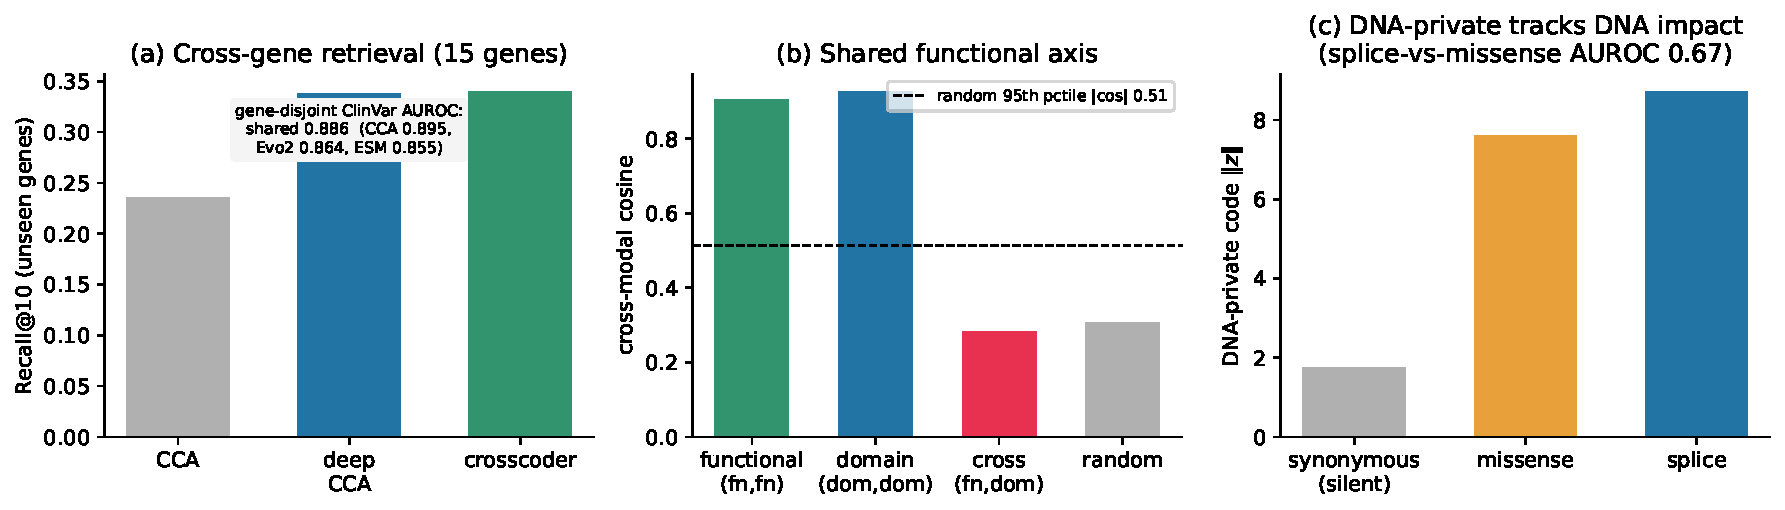
\includegraphics[width=\linewidth]{../figures/fig_extra.pdf}
\caption{\textbf{Generalization, shared axis, and specialization.} (a)~On a 15-gene ClinVar
panel, the alignment transfers to \emph{unseen} genes (Recall@10 within held-out genes; box:
gene-disjoint pathogenicity AUROC). (b)~Functional and domain directions align across modalities
(cosine $\gg$ random), and are property-specific (functional vs.\ domain is at the random level).
(c)~Applied to variant classes it never trained on, the DNA-private code's activation tracks
DNA-level severity: splice $>$ missense $\gg$ synonymous (silent).}
\label{fig:extra}
\end{figure}

\section{Extension: model-diffing a disease fine-tune (DeltaEvo)}
\label{sec:c}
The same delta framework diffs a model against a fine-tuned copy of itself. We LoRA-fine-tune
Evo\,2 \citep{hu2022lora} (rank-8 adapters on the MLPs of blocks 20--26, backbone frozen) to
classify BRCA1 loss-of-function from its variant-position delta activation, on the
domain-disjoint split. (Evo\,2's inference stack stores weights as \emph{inference tensors} that
cannot be differentiated; we re-materialise them to enable LoRA autograd---a small reusable
recipe.) Fine-tuning improves held-out RING LOF classification from AUROC \cBaseOOD{} (frozen
backbone + head) to \cLoraOOD{} (LoRA), and the adaptation lives in the backbone: a frozen head
on the \emph{fine-tuned} activations already reaches \cFtOOD{}, and the mean per-variant
activation change is $\lVert\Delta_{\mathrm{ft}}-\Delta_{\mathrm{base}}\rVert=\cDiffNorm{}$ (not a
head-only shortcut). Training a Delta-Crosscoder on the matched pairs, it reconstructs the
base$\to$ft \emph{difference} better than a standard crosscoder ($\Delta$FVE $+\cDeltaAdv{}$), and
its taxonomy has \cShared{} shared and \cAmplified{} \emph{amplified} latents but \cFtSpecific{}
fine-tune-\emph{specific} ones: narrow disease fine-tuning amplifies existing features rather than
introducing new ones. The amplified latents are only weakly LOF-selective (AUROC \cLofAmp{}),
leaving open which reweighted features drive the gain---a preliminary but encouraging
demonstration that Delta-Crosscoders can audit genomic-LM fine-tuning.

\section{Discussion and limitations}
We are deliberately explicit about what does and does not work. \textbf{(i)~Method is a setting,
not a new architecture.} The alignment is a deep-CCA; the sparse dictionaries add interpretability
and diffing. Our ablation shows the sparse codes do \emph{not} improve alignment
(they retrieve at chance), so the headline retrieval/DMS gains should be read as ``learned
cross-modal alignment of variant deltas beats linear CCA,'' with the crosscoder contributing the
interpretable codes and the shared-axis and diffing analyses. \textbf{(ii)~Assay coverage.} The
DMS-level analysis is on BRCA1 (to remove the gene-identity confound); we show cross-gene transfer
on 15 ClinVar genes, but extending the continuous-DMS analysis to many assays (e.g.\ ProteinGym
\citep{notin2023proteingym}) is the natural next step. \textbf{(iii)~Not a SOTA predictor.} The
shared code beats CCA and the DNA probe, but ESM-2 alone predicts missense DMS better; the value
is interpretability, cross-modal retrieval, transfer, and the shared-axis result---not raw
accuracy. \textbf{(iv)~Representation- vs latent-level interpretability.} The shared
\emph{representation} predicts LOF and domain, but individual sparse latents are only weakly
annotation-selective, so we report collective probes rather than claim monosemantic features.
\textbf{(v)~Alignment $\neq$ causal exchange.} Representational alignment (cosine \cosDms{}) does
not translate into a causal handle: injecting the shared functional direction is non-specific in
Evo\,2 and only a marginal, non-significant trend in ESM-2. This may reflect the difficulty of
steering Evo\,2's long-convolutional stack with a single-position edit as much as an absence of
shared causal structure, and deserves dedicated study with richer interventions.

\section{Conclusion}
Do genomic and protein language models share variant mechanisms? At the level of
\emph{representations}, partly yes: a learned alignment of paired variant deltas beats linear CCA,
transfers to unseen genes and domains, and places the two models' functional directions on the
same axis. At the level of \emph{individual causal features}, not demonstrably: sparse latents are
weakly monosemantic and the shared direction is not an interchangeable causal handle. Measuring
this honestly---across the central dogma, with proper controls and negative results---is, we
argue, a useful step toward cross-modal mechanistic interpretability of biological foundation
models.

\small
\bibliographystyle{plainnat}
\bibliography{refs}
\end{document}
